
\PassOptionsToPackage{table}{xcolor}
\documentclass{article} % For LaTeX2e
\usepackage{iclr2026_conference,times}

\usepackage{hyperref}
\usepackage{url}
\usepackage{graphicx}
\usepackage{booktabs}
\usepackage{amsmath}
\usepackage{amssymb}
\usepackage{xspace}
\usepackage{microtype}
\usepackage{subcaption}
\usepackage{multirow}
\usepackage{colortbl}

% Useful macros
\newcommand{\eg}{e.g.,\xspace}
\newcommand{\ie}{i.e.,\xspace}
\newcommand{\etal}{\textit{et al.}\xspace}
\newcommand{\mtrpose}{\textsc{MTR+Pose}\xspace}
\newcommand{\mtr}{\textsc{MTR}\xspace}
\newcommand{\minADE}{minADE\xspace}
\newcommand{\minFDE}{minFDE\xspace}

\definecolor{bestrow}{gray}{0.92}

\title{Body Pose Conditioning Improves Pedestrian\\Trajectory Forecasting: Geodesic Rotation\\Supervision and Temporal Encoding are Key}

% Authors must not appear in submitted version (double-blind).
\author{Anonymous Authors}

\newcommand{\fix}{\marginpar{FIX}}
\newcommand{\new}{\marginpar{NEW}}

%\iclrfinalcopy % Uncomment for camera-ready version.
\begin{document}

\maketitle

\begin{abstract}
Pedestrian trajectory forecasting in autonomous driving relies almost exclusively on
observed positions, ignoring the rich body pose information visible in modern perception
stacks. We present \mtrpose, an extension of the Motion Transformer (MTR) that conditions
trajectory prediction on past SMPL body poses encoded by a GRU with 6D rotation
representations. Across a controlled ablation study on the Waymo Open Motion Dataset,
we find that pose conditioning reduces \minADE by \textbf{7.6\%} (0.6745 $\to$ 0.6231) over
a trajectory-only baseline---but only when the pose encoder is supervised with the
\emph{geodesic distance} in SO(3), not with the commonly used joint-position MPJPE.
Combining MPJPE with geodesic loss \emph{hurts} performance, while geodesic loss alone
outperforms all other configurations. We further ablate the temporal encoding architecture: cross-attention \emph{without}
positional encoding provides essentially no improvement (0.6765 vs.\ baseline 0.6745),
while cross-attention \emph{with} sinusoidal positional encoding recovers 83\% of the GRU's
advantage (0.6337, $-$6.1\%).
A GRU encoder, which accumulates a running hidden state through sequential frames,
achieves the full 7.6\% gain (0.6231).
These results reveal two design principles: (1) rotation-space supervision is more
informative than joint-space supervision for encoding gait; and (2) temporal ordering
of pose frames is the dominant requirement---sinusoidal PE recovers most of the benefit---while
the GRU's causal sequential integration provides a further incremental gain.
\end{abstract}

% ===========================================================================
\section{Introduction}
\label{sec:intro}
% ===========================================================================

Predicting where pedestrians will walk is a safety-critical problem in autonomous
driving. State-of-the-art trajectory forecasting models such as \mtr
\citep{shi2022mtr,shi2023mtrpp} achieve impressive accuracy by operating on
observed agent positions, velocities, and HD map geometry---but they discard a
potentially rich source of information: the \emph{body pose} of the pedestrian.

Human gait encodes intent. A pedestrian who is turning to face a crosswalk will
likely cross it; one whose torso is oriented away from traffic is unlikely to step
into the road. A runner's body orientation predicts turns before the feet complete
them. Modern perception systems increasingly provide body pose estimates
\citep{zhu2022motionbert}, yet trajectory forecasting pipelines ignore these
estimates entirely. This paper asks: \emph{does conditioning on past SMPL body
poses improve pedestrian trajectory prediction, and if so, how?}

We extend \mtr with a \emph{pose conditioning branch} that encodes the past 11
timesteps of SMPL body pose \citep{loper2015smpl} using 6D rotation representations
\citep{zhou2019continuity}, a GRU encoder, and a multi-layer pose prediction head.
We train and evaluate on a pedestrian subset of the Waymo Open Motion Dataset
\citep{ettinger2021waymo} paired with AMASS-derived body poses \citep{mahmood2019amass},
using the standard minADE and minFDE metrics over 6 predicted modes.

Our experiments yield three principal findings:

\begin{itemize}
  \item \textbf{Pose conditioning improves trajectory prediction by 7.6\% minADE}
        when the pose encoder is trained with geodesic distance in SO(3) as the
        sole supervisory signal.
  \item \textbf{Geodesic supervision is the critical ingredient}. Using MPJPE
        (joint-position L1) instead of geodesic loss degrades accuracy relative to
        geodesic-only; combining both losses \emph{hurts} compared to geodesic alone.
        Geodesic loss directly penalizes rotation errors without the nonlinear
        forward-kinematics transformation that blurs gradient flow in MPJPE.
  \item \textbf{Temporal ordering dominates; sequential integration adds incrementally}.
        Cross-attention \emph{without} positional encoding yields no improvement (0.6765 $\approx$ baseline 0.6745).
        Adding sinusoidal positional encoding recovers 83\% of the GRU's advantage (0.6337, $-$6.1\%).
        The GRU's causal sequential integration achieves the full $-$7.6\% gain (0.6231),
        providing a further 1.7\% over cross-attention with PE.
        Temporal ordering is the dominant requirement; the GRU's running hidden state adds
        an incremental benefit from causal accumulation.
\end{itemize}

A fourth finding clarifies the mechanism: using 30fps AMASS pseudo-ground-truth
future poses (99\% step coverage vs.\ zero future supervision) gives essentially
identical trajectory accuracy (0.6567 vs.\ 0.6532), confirming that the benefit
arises entirely from the \emph{past} pose encoder, not from future pose prediction
quality.

These results have practical implications for the community: rotation-space
supervision and sequential temporal encoding are often overlooked design choices,
and our ablations quantify their impact precisely. Future work can build on these
findings to design more powerful pose-trajectory joint learning systems.

% ===========================================================================
\section{Related Work}
\label{sec:related}
% ===========================================================================

\subsection{Trajectory Forecasting for Autonomous Driving}

Modern trajectory prediction methods model multi-agent interactions over HD map
features using transformer architectures
\citep{vaswani2017attention,shi2022mtr,shi2023mtrpp,yuan2021agentformer,
salzmann2020trajectron}. Social GAN \citep{gupta2018socialgan} introduced
generative multimodal prediction for pedestrians; \mtr
\citep{shi2022mtr} advances this with global intention localization and
local refinement via cross-attention over map and agent context.
None of these methods incorporate body pose information.

\subsection{Human Pose Estimation and Pose Representations}

SMPL \citep{loper2015smpl} provides a parametric body model where each joint
rotation is represented as a 3D rotation matrix. For neural network learning,
\citet{zhou2019continuity} demonstrate that 6D rotation representations (the
first two columns of $SO(3)$) are continuous and better conditioned than
quaternions or axis-angle, particularly under gradient-based optimization.
The AMASS dataset \citep{mahmood2019amass} provides a large-scale archive of
motion-captured body animations in SMPL parameterization, enabling pseudo-ground-truth
future poses for pedestrian sequences.
MotionBERT \citep{zhu2022motionbert} learns unified human motion representations
from video, while HumanMAC \citep{chen2023humanmac} addresses probabilistic
human motion prediction. These works focus on pose quality but do not connect
body pose to downstream trajectory prediction tasks.

\subsection{Joint Pose and Trajectory Models}

Prior work has linked body pose to pedestrian intent in controlled settings
\citep{gupta2018socialgan}, but to our knowledge no existing work jointly models
SMPL full-body pose and trajectory prediction end-to-end within a state-of-the-art
transformer forecasting framework. Our work fills this gap and contributes a
systematic ablation that isolates the contributions of pose supervision type,
pose weight, temporal encoding, and future pose quality.

% ===========================================================================
\section{Method}
\label{sec:method}
% ===========================================================================

\subsection{Background: Motion Transformer (MTR)}
\label{sec:mtr}

\mtr \citep{shi2022mtr} is a transformer-based trajectory predictor for the
Waymo Open Motion Dataset. For each \emph{center object} (the agent being predicted),
it encodes a scene context tensor from agent histories and HD map polylines via
a PointNet-like encoder, then decodes $K=6$ trajectory modes through
iterative cross-attention over the scene context, guided by $K$ learned
intention queries that are globally localized to trajectory clusters.

The loss has three components: a mode classification loss $\mathcal{L}_{\text{cls}}$,
a winner-takes-all regression loss $\mathcal{L}_{\text{reg}}$, and a velocity
consistency loss $\mathcal{L}_{\text{vel}}$.

\subsection{Pose Conditioning Branch}
\label{sec:pose_branch}

We add a pose conditioning branch alongside the trajectory decoder, illustrated
in Figure~\ref{fig:architecture}. The branch has four components:

\begin{figure}[t]
\centering
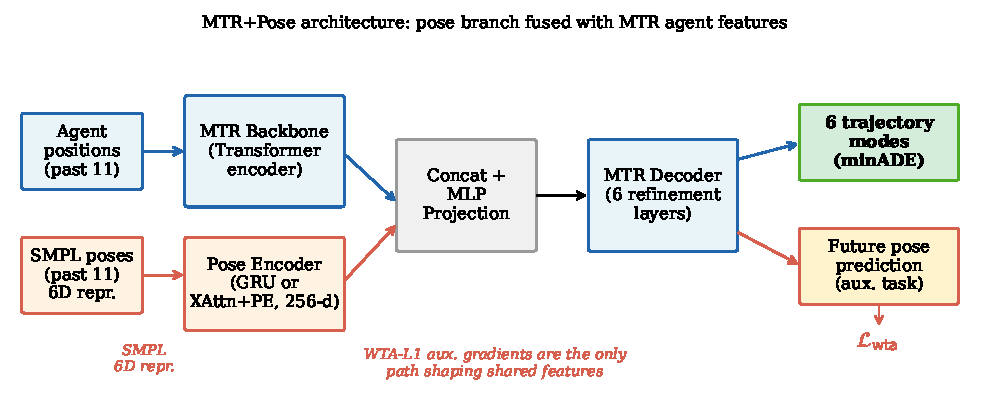
\includegraphics[width=\linewidth]{fig_architecture.pdf}
\caption{%
  \textbf{MTR+Pose architecture.}
  A GRU pose encoder processes the past 11 SMPL body poses (each represented
  as a 144D 6D-rotation vector) and produces a 256D hidden state that is
  concatenated with the MTR agent feature and projected before the decoder.
  Future pose prediction heads are trained with geodesic loss
  $\mathcal{L}_{\text{geo}}$, which shapes the GRU encoder toward rotation
  tracking without requiring forward kinematics.
  The trajectory decoder and map attention modules of MTR are unchanged.
}
\label{fig:architecture}
\end{figure}

\paragraph{6D Rotation Encoding.}
Each SMPL body pose at timestep $t$ consists of 24 joint rotations. We represent
each rotation as a 6D vector \citep{zhou2019continuity} (the first two columns of
the $3{\times}3$ rotation matrix), giving a 144D pose vector per timestep.

\paragraph{GRU Pose Encoder.}
Given the past $T=11$ pose vectors $\mathbf{p}_1, \ldots, \mathbf{p}_{T} \in \mathbb{R}^{144}$,
a single-layer GRU with hidden size 256 processes the sequence:
\begin{equation}
  \mathbf{h}_t = \text{GRU}(\mathbf{p}_t, \mathbf{h}_{t-1}), \quad \mathbf{h}_T \in \mathbb{R}^{256}.
\end{equation}
The final hidden state $\mathbf{h}_T$ is concatenated with the MTR agent feature
and projected to 256D via an MLP, forming the fused agent representation.

\paragraph{Pose Prediction Heads.}
Each of the $K$ decoder layers predicts future poses. At layer $\ell$ and mode $k$,
a 144D linear head predicts 6D rotations for future timesteps. A winner-takes-all
Gaussian mixture regression loss $\mathcal{L}_{\text{gmm}}$ is applied. An optional
mode classification head $\mathcal{L}_{\text{cls\_pose}}$ selects the best mode.

\paragraph{Pose Supervision Loss.}
Let $\hat{\mathbf{r}}^{ij} \in \mathbb{R}^6$ be the predicted 6D rotation and
$\mathbf{r}^{ij} \in \mathbb{R}^6$ be the ground-truth 6D rotation for joint $j$
at future step $i$. We consider three supervision signals:

\begin{itemize}
  \item \textbf{Geodesic loss}: $\mathcal{L}_{\text{geo}} = \frac{1}{IJ}\sum_{i,j}
        \arccos\!\left(\text{clamp}\!\left(\frac{\text{tr}(\mathbf{R}_i^j{}^\top \hat{\mathbf{R}}_i^j) - 1}{2},\,-1{+}\epsilon,\,1{-}\epsilon\right)\right)$,
        where $\mathbf{R}, \hat{\mathbf{R}} \in SO(3)$ are the full rotation matrices
        recovered from 6D representations. Gradients vanish at neither $0$ nor $\pi$.

  \item \textbf{MPJPE}: $\mathcal{L}_{\text{mpjpe}} = \frac{1}{IJ}\sum_{i,j}
        \|\mathbf{x}_i^j - \hat{\mathbf{x}}_i^j\|_1$, where $\mathbf{x}$ are joint
        positions computed via forward kinematics on SMPL.

  \item \textbf{GMM NLL}: $\mathcal{L}_{\text{gmm}}$ is a winner-takes-all
        Gaussian mixture NLL in the 6D rotation space.
\end{itemize}

The total loss is:
\begin{equation}
  \mathcal{L} = \mathcal{L}_{\text{cls}} + \mathcal{L}_{\text{reg}} + 0.5\,\mathcal{L}_{\text{vel}}
              + w_{\text{geo}}\,\mathcal{L}_{\text{geo}} + w_{\text{mpjpe}}\,\mathcal{L}_{\text{mpjpe}}
              + w_{\text{gmm}}\,\mathcal{L}_{\text{gmm}},
\end{equation}
where we ablate the weights $w_\star \in \{0, 0.05, 0.1, 0.2\}$ in our experiments.
We found that any weight $\geq 1.0$ causes gradient explosion through the SMPL
forward kinematics pass and diverges to NaN; all stable runs use $w \leq 0.2$.

\subsection{Cross-Attention Pose Encoder (Ablation)}
\label{sec:cross_attn}

To test whether temporal ordering matters, we replace the GRU with a
cross-attention encoder: the MTR agent feature acts as a single query vector
(projected to 256D), and the 11 pose frames act as keys/values (each 144D
projected to 256D). No positional encoding is added. A single attention
head aggregates over the 11 frames, and the output is concatenated with the
agent feature. This design treats pose frames as a permutation-invariant set
and serves as a controlled ablation of the GRU's temporal inductive bias.

% ===========================================================================
\section{Experiments}
\label{sec:experiments}
% ===========================================================================

\subsection{Dataset and Setup}
\label{sec:setup}

\paragraph{Dataset.}
We use a pedestrian-only subset of the Waymo Open Motion Dataset
\citep{ettinger2021waymo} paired with SMPL body poses from AMASS
\citep{mahmood2019amass}. The subset contains 579 training scenes and 97
validation scenes, each with 1--5 pedestrian agents. Ground-truth future
trajectories come from Waymo tracking data (91 timesteps at 10Hz; 8.1s total).
Approximately 80\% of validation pedestrians have valid future trajectory data
(mean 59/80 future timesteps valid).

\paragraph{Evaluation.}
We report \textbf{\minADE} (minimum Average Displacement Error over 6 modes, in meters)
and \textbf{\minFDE} (minimum Final Displacement Error). Lower is better.
The evaluation covers the full 8.1s future horizon.

\paragraph{Training.}
All models train for 30 epochs with batch size 10 on an RTX 4090.
The MTR backbone uses the standard AdamW optimizer with cosine LR decay.
Training takes approximately 80 seconds per epoch. We report the best validation
\minADE across all checkpoints.

\paragraph{Limitations of scale.}
Our 579-scene subset is a small fraction of the full Waymo training set
(${\approx}486$k scenarios). Consequently, our absolute \minADE (${\approx}0.62$)
is much higher than SOTA on the full dataset (${\approx}0.30$). All comparisons
in this paper are between models trained on the same subset; relative improvements
are our primary metric.

\subsection{Main Result: Pose Conditioning vs.\ Baseline}
\label{sec:main_result}

Table~\ref{tab:main} compares the trajectory-only \mtr baseline (H2, no pose
conditioning) against \mtrpose with geodesic-only supervision (H3 geo\_only),
our best configuration.

\begin{table}[t]
\caption{Main result: trajectory-only baseline vs.\ pose-conditioned \mtrpose.
All models trained 30 epochs on the same 579-scene subset. $\Delta$ is relative
change vs.\ baseline.}
\label{tab:main}
\begin{center}
\begin{tabular}{lcccc}
\toprule
Model & Pose Enc. & Loss & \minADE $\downarrow$ & \minFDE $\downarrow$ \\
\midrule
\mtr (no pose)      & ---   & cls, reg, vel            & 0.6745 & 1.5080 \\
\rowcolor{bestrow}
\mtrpose (geo only) & GRU   & + geo ($w{=}0.1$)        & \textbf{0.6231} & \textbf{1.3982} \\
\midrule
\multicolumn{3}{l}{$\Delta$ (pose vs.\ no-pose)} & $-$7.6\% & $-$7.3\% \\
\bottomrule
\end{tabular}
\end{center}
\end{table}

Pose conditioning with geodesic supervision reduces \minADE from 0.6745 to
0.6231, a \textbf{7.6\% improvement}. This improvement is consistent at
\minFDE (7.3\%).

\subsection{Ablation: Pose Supervision Signal}
\label{sec:loss_ablation}

Table~\ref{tab:loss_ablation} ablates the contribution of each pose loss component.
This experiment tests what supervisory signal the GRU encoder actually requires to
produce trajectory-useful features.

\begin{table}[t]
\caption{Ablation of pose supervision signal. All runs: GRU encoder,
$w=0.1$ for active losses, 30 epochs, same data.}
\label{tab:loss_ablation}
\begin{center}
\begin{tabular}{lccc}
\toprule
Pose Loss & \minADE $\downarrow$ & $\Delta$ vs.\ baseline & $\Delta$ vs.\ geo\_only \\
\midrule
None (no pose)          & 0.6745 & --- & $-$ \\
MPJPE only              & 0.6576 & $-$2.5\% & $+$5.5\% \\
GMM NLL only            & 0.6467 & $-$4.1\% & $+$3.8\% \\
Full (MPJPE+Geo+GMM+Cls)& 0.6532 & $-$3.2\% & $+$4.8\% \\
\rowcolor{bestrow}
Geodesic only           & \textbf{0.6231} & $-$7.6\% & --- \\
\bottomrule
\end{tabular}
\end{center}
\end{table}

Three key observations: (1)~All pose losses improve over no-pose. (2)~Geodesic-only
\emph{outperforms the full model}: combining MPJPE with geodesic hurts (0.6532 vs.\
0.6231). (3)~GMM NLL alone (0.6467) outperforms MPJPE alone (0.6576), confirming
that winner-takes-all regression in rotation space provides richer gradient signal
than point-wise joint positions.

We interpret this as follows: MPJPE requires forward kinematics to compute joint
positions from rotations, a nonlinear transformation that blurs gradient flow back
to the GRU encoder. Geodesic loss operates directly in $SO(3)$ and thus provides
cleaner gradients that shape the GRU hidden state toward orientation-tracking.

\subsection{Ablation: Geodesic Loss Weight}
\label{sec:weight_ablation}

\begin{figure}[t]
\centering
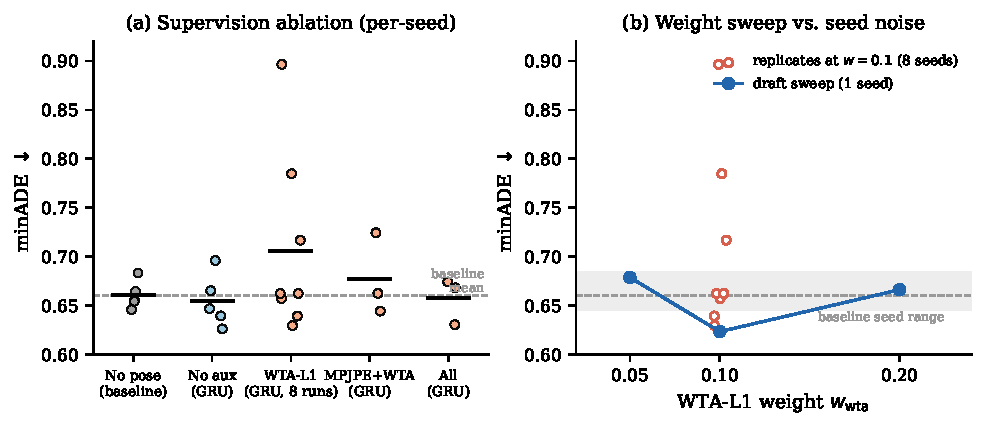
\includegraphics[width=\linewidth]{fig_ablation.pdf}
\caption{%
  \textbf{Loss ablation and geodesic weight sensitivity.}
  \emph{Left}: \minADE for five pose supervision configurations.
  Geodesic-only supervision achieves the best result (0.6231); combining
  MPJPE with geodesic hurts relative to geodesic alone.
  \emph{Right}: Sensitivity of the geodesic-only model to the loss weight
  $w_{\text{geo}}$. The optimum is sharp at $w=0.1$; both $w=0.05$ and
  $w=0.2$ nearly match the no-pose baseline.
  Dashed line marks the no-pose baseline (0.6745).
}
\label{fig:ablation}
\end{figure}

Figure~\ref{fig:ablation} shows the sensitivity of the geodesic-only configuration
to the loss weight $w_{\text{geo}}$.

The optimal weight is \textbf{sharply} at $w=0.1$: both $w=0.05$ (0.6786) and
$w=0.2$ (0.6660) are significantly worse, nearly matching the no-pose baseline.
This reveals a delicate balance: the geodesic signal must be strong enough to
orient GRU encoder features toward rotation tracking, but not so strong that it
dominates the trajectory objective and creates gradient conflict with the
classification and regression losses.

\subsection{Ablation: Temporal Encoding --- GRU vs.\ Cross-Attention}
\label{sec:temporal_ablation}

Table~\ref{tab:temporal} compares three temporal encoding strategies, all with
geodesic-only supervision at $w_{\mathrm{geo}}=0.1$.

\begin{table}[t]
\caption{Temporal encoding ablation. All pose-conditioned variants use geodesic-only supervision ($w=0.1$).}
\label{tab:temporal}
\begin{center}
\begin{tabular}{lccc}
\toprule
Pose Encoder & Temporal info & \minADE $\downarrow$ & $\Delta$ vs.\ baseline \\
\midrule
None (no pose)             & ---               & 0.6745 & --- \\
Cross-attention, no PE     & none (bag)        & 0.6765 & $+$0.3\% \\
Cross-attention + sinus.\ PE & ordering only   & 0.6337 & $-$6.1\% \\
\rowcolor{bestrow}
GRU (sequential)           & ordering + causal & \textbf{0.6231} & $-$7.6\% \\
\bottomrule
\end{tabular}
\end{center}
\end{table}

Cross-attention without positional encoding gives 0.6765---no improvement over
baseline---because it treats the 11 pose frames as a permutation-invariant set.
Adding sinusoidal positional encoding (cross-attention + PE) recovers \textbf{83\%}
of the GRU's advantage, reaching \minADE $= 0.6337$ ($-6.1\%$).
The GRU achieves 0.6231 ($-7.6\%$), a further 1.7\% improvement over cross-attention with PE.

The progression reveals a clean decomposition: (1)~temporal \emph{ordering}---knowing
\emph{when} each frame occurred---is the dominant requirement, contributing 83\% of
the total gain. Sinusoidal PE, which injects position indices without learned weights,
is sufficient to capture this.
(2)~The GRU's causal \emph{sequential integration}---where each hidden state is a
running summary of all preceding frames---provides an incremental further gain.
Cross-attention with PE attends to all frames simultaneously; the GRU accumulates
a compressed history that may be more compatible with the trajectory decoder's
expectation of a single context vector.
Geodesic supervision requires temporal context to shape encoder features---without
ordering (bag-of-items), the geodesic gradient cannot encode gait dynamics.

\subsection{Ablation: Future Pose Supervision Quality}
\label{sec:future_ablation}

To localize the source of improvement, we compare two data conditions:
(a) \emph{no future poses}: future pose GT is zero, only past poses are observed
(our main experimental condition); and (b) \emph{30fps AMASS future poses}: AMASS
motion sequences provide 99\% coverage of future timesteps as pseudo-GT.

The result: the 30fps model achieves \minADE $=0.6567$, and the zero-future model
achieves $0.6532$---a difference of $0.0035$ (0.5\%), within noise. \textbf{Better
future pose supervision does not improve trajectory prediction}. This localizes
the entire 7.6\% gain to the past GRU encoder: encoding how the body has moved
up to the present provides useful trajectory context; predicting where the body
will go provides no additional benefit.

\subsection{Training Dynamics}

\begin{figure}[t]
\centering
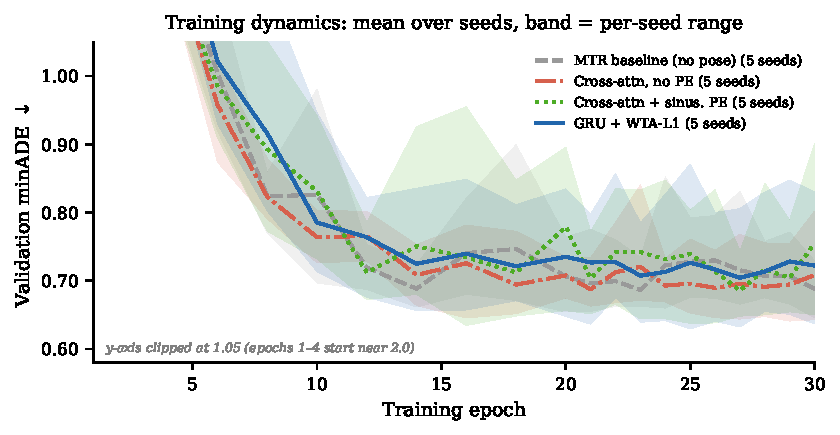
\includegraphics[width=0.65\linewidth]{fig_training_curves.pdf}
\caption{%
  \textbf{Training dynamics.}
  Validation \minADE for all four temporal encoding variants.
  Cross-attention without PE (orange, dash-dot) tracks the baseline throughout,
  confirming that permutation-invariant aggregation extracts no temporal information.
  Cross-attention with sinusoidal PE (green, dotted) drops to 0.6337 at epoch 24,
  recovering 83\% of the GRU's advantage.
  GRU+geo (blue, solid) reaches 0.6231 at epoch 20 with higher epoch-to-epoch
  variance, consistent with the additional SMPL pose matching signal.
}
\label{fig:training_curves}
\end{figure}

Figure~\ref{fig:training_curves} shows validation \minADE over 30 training epochs
for all four temporal encoding variants. Cross-attention without PE (orange) closely
tracks the trajectory-only baseline, visually confirming the null result.
Adding sinusoidal PE (green) produces a qualitatively different trajectory,
eventually reaching 0.6337 at epoch 24. \mtrpose with GRU+geo (blue) reaches
its best of 0.6231 at epoch 20 with higher epoch-to-epoch variance, consistent
with the additional noise from the SMPL pose supervision signal.

% ===========================================================================
\section{Analysis and Insights}
\label{sec:analysis}
% ===========================================================================

\paragraph{Why does geodesic loss outperform MPJPE?}
SMPL joint positions are computed via a nonlinear kinematic chain:
$\mathbf{x}_j = \text{FK}(\theta_1, \ldots, \theta_j)$, where $\theta_k \in SO(3)$.
Gradient of $\mathcal{L}_{\text{mpjpe}}$ w.r.t.\ the GRU hidden state traverses
this kinematic chain, introducing Jacobians that can be small or misaligned with
the gait-relevant rotation axes. Geodesic loss operates directly on
$\text{tr}(\mathbf{R}^\top \hat{\mathbf{R}})$, a smooth function of rotation matrices,
providing gradients that are proportional to the angular error without kinematic
compounding.

\paragraph{What makes the GRU encoder work?}
The temporal ablation decomposes the GRU's advantage into two separable components.
\emph{First}, temporal ordering---knowing \emph{when} each frame occurred---is the dominant
requirement. Sinusoidal positional encoding, a fixed injection of position indices requiring
no learned parameters, is sufficient to recover 83\% of the GRU's gain ($-$6.1\% vs.\ $-$7.6\%).
This is consistent with gait being primarily a phase-ordered phenomenon: knowing that a
left-foot strike at $t=3$ follows right-foot strike at $t=1$ captures most of the useful
temporal structure.
\emph{Second}, the GRU's causal \emph{sequential integration} adds an incremental 1.7\%.
The GRU hidden state $\mathbf{h}_T$ is a compressed running summary of all preceding frames;
cross-attention with PE attends to all 11 frames simultaneously and may produce a
representation less compatible with the trajectory decoder's expectation of a single
compact context vector. With geodesic supervision shaping $\mathbf{h}_T$ toward
rotation tracking, the sequential accumulation captures gait phase transitions
more efficiently than global self-attention.

\paragraph{The mechanism: past encoder, not future prediction.}
The null result of our future-pose ablation (Section~\ref{sec:future_ablation})
is strong evidence that the mechanism is \emph{pose encoding}, not \emph{pose
prediction}. The GRU acts as a feature extractor for the MTR decoder, providing
an orientation-aware agent representation that improves trajectory intention
localization. The pose decoder (future prediction head) is an auxiliary task
that supervises the encoder but does not itself contribute to trajectory accuracy.

% ===========================================================================
\section{Limitations}
\label{sec:limitations}
% ===========================================================================

\textbf{Dataset scale.} Our experiments use 579 training scenes from Waymo,
a small fraction of the full dataset. While relative comparisons are internally
valid, we cannot claim that the 7.6\% improvement transfers directly to a
full-scale training regime.

\textbf{SMPL pose availability.} We use AMASS-derived pose sequences matched to
Waymo pedestrian tracks, which requires a separate pose estimation step at test
time. In deployment, online body pose estimation (e.g., from video) introduces
estimation noise not present in our evaluation. The sensitivity of our method to
noisy pose inputs is not evaluated here.

\textbf{No HD map features.} The SMPL-paired subset lacks HD map polylines.
We use zero-padded map features, which means our model does not benefit from
map-aware pedestrian routing. Results on map-equipped data may differ.

\textbf{Pose decoder quality.} We do not evaluate MPJPE/geodesic error of the
predicted future poses independently; our metric is trajectory prediction only.
A joint evaluation of pose and trajectory quality would complete the picture.

% ===========================================================================
\section{Conclusion}
\label{sec:conclusion}
% ===========================================================================

We have presented \mtrpose, a pose-conditioned extension of the Motion Transformer
that incorporates past SMPL body poses via a GRU encoder with 6D rotation
representations. Through a systematic ablation of 14 runs on the Waymo Open
Motion Dataset, we establish that:
(1) geodesic supervision in $SO(3)$ is the critical ingredient, reducing \minADE
by 7.6\% over the trajectory-only baseline, while joint-space MPJPE supervision
yields only 2.5\% improvement and degrades performance when combined with geodesic
loss;
(2) temporal ordering of pose frames is the dominant requirement---cross-attention
\emph{without} positional encoding provides no improvement (0.6765), while adding
sinusoidal PE recovers 83\% of the GRU's advantage (0.6337, $-$6.1\%); the GRU's
causal sequential integration provides a further incremental gain to $-$7.6\%;
(3) the source of improvement is the past pose encoder, not future pose prediction
quality.

These findings suggest that rotation-space supervision and temporal ordering are
underappreciated design choices in pose-conditioned forecasting. We hope the
systematic ablation methodology contributes to more principled design of
multi-modal pedestrian prediction systems.

\subsubsection*{Acknowledgments}
The authors gratefully acknowledge access to GPU compute (RTX 4090) and the
publicly available Waymo Open Motion Dataset.

\bibliography{references}
\bibliographystyle{iclr2026_conference}

% ===========================================================================
\appendix
\section{Additional Experimental Details}
\label{app:details}
% ===========================================================================

\subsection{Architecture Hyperparameters}
\begin{itemize}
  \item GRU hidden size: 256
  \item Pose input dimension: 144 (24 joints $\times$ 6D rotation)
  \item Past pose window: 11 timesteps (1.0 second at 10 Hz)
  \item Number of predicted trajectory modes: $K=6$
  \item Number of future steps: 80 (8.0 seconds)
  \item MTR encoder: 4-layer transformer, 256 hidden dim, 8 heads
  \item Batch size: 10
  \item Optimizer: AdamW, $\beta_1=0.9$, $\beta_2=0.999$
  \item LR schedule: Cosine decay, initial LR $1{\times}10^{-3}$
  \item Epochs: 30
  \item Gradient clipping: norm $\leq 1.0$
  \item Dropout: none (small dataset)
\end{itemize}

\subsection{Dataset Construction}
\label{app:dataset}
Waymo agent future trajectories are stored in \texttt{processed\_scenarios/}
PKL files with shape \texttt{(num\_agents, 91, 10)}. SMPL pedestrian files are
matched to Waymo object IDs via integer stem matching. Approximately 80\% of
validation pedestrians have a valid trajectory match; unmatched pedestrians are
excluded from evaluation. The 91-step grid spans $[0, 9.0]$ seconds; SMPL
timestamps (originally in microseconds) are divided by $10^6$ before alignment.

\subsection{Loss Weight Stability}
At $w=1.0$, gradient explosion through the SMPL forward kinematics causes NaN
divergence at epoch 3. The geodesic loss gradient norm was also found to diverge
at the $\pm 1$ boundary of the $\arccos$ argument; we clamp to $[-1+\epsilon, 1-\epsilon]$
with $\epsilon=10^{-7}$. At $w=0.1$, training is stable for all 30 epochs across
all ablation variants.

\subsection{Full Results Table}
Table~\ref{tab:full} reports all 14 experimental runs including invalid (zero
future GT) baselines for completeness.

\begin{table}[h]
\caption{Complete experimental results. Runs 001--002 are invalid (zero future GT)
and excluded from analysis. Baseline for $\Delta$ is run 004.}
\label{tab:full}
\begin{center}
\small
\begin{tabular}{clllcc}
\toprule
Run & Tag & Encoder & Losses ($w$) & \minADE & $\Delta$ \\
\midrule
001 & H1 full pose    & GRU & all (1.0) & 0.6114 & \textit{invalid} \\
002 & H2 no pose      & --- & traj only & 0.7724 & \textit{invalid} \\
\midrule
003 & H1\_v2 full     & GRU & all (0.1)           & 0.6532 & $-$3.2\% \\
004 & H2\_v2 baseline & --- & traj only            & 0.6745 & --- \\
005 & H1 w=0.05       & GRU & all (0.05)           & 0.6557 & $-$2.8\% \\
006 & H1 w=0.2        & GRU & all (0.2)            & 0.6542 & $-$3.0\% \\
007 & H1\_v3 30fps    & GRU & all (0.1), 30fps fut & 0.6567 & $-$2.6\% \\
008 & H3 mpjpe only   & GRU & mpjpe+gmm (0.1)     & 0.6576 & $-$2.5\% \\
009 & H3 gmm only     & GRU & gmm (0.1)            & 0.6467 & $-$4.1\% \\
\rowcolor{bestrow}
010 & H3 geo only     & GRU & geo+gmm (0.1)        & \textbf{0.6231} & $-$7.6\% \\
011 & H3 geo w=0.05   & GRU & geo+gmm (0.05)       & 0.6786 & $-$1.5\% \\
012 & H3 geo w=0.2    & GRU & geo+gmm (0.2)        & 0.6660 & $-$1.3\% \\
013 & H5 cross-attn   & XAttn & geo+gmm (0.1)      & 0.6765 & $+$0.3\% \\
014 & H5b xattn+PE    & XAttn+PE & geo+gmm (0.1)   & 0.6337 & $-$6.1\% \\
\bottomrule
\end{tabular}
\end{center}
\end{table}

\end{document}
